%%%%%%%%%%%%%%%%%%%%%%%%%%%%%%%%%%%%%%%%%
% Wenneker Article
% LaTeX Template
% Version 2.0 (28/2/17)
%
% This template was downloaded from:
% http://www.LaTeXTemplates.com
%
% Authors:
% Vel (vel@LaTeXTemplates.com)
% Frits Wenneker
%
% License:
% CC BY-NC-SA 3.0 (http://creativecommons.org/licenses/by-nc-sa/3.0/)
%
%%%%%%%%%%%%%%%%%%%%%%%%%%%%%%%%%%%%%%%%%

%----------------------------------------------------------------------------------------
%	PACKAGES AND OTHER DOCUMENT CONFIGURATIONS
%----------------------------------------------------------------------------------------

\documentclass[10pt, a4paper, twocolumn]{article} % 10pt font size (11 and 12 also possible), A4 paper (letterpaper for US letter) and two column layout (remove for one column)

%%%%%%%%%%%%%%%%%%%%%%%%%%%%%%%%%%%%%%%%%
% Wenneker Article
% Structure Specification File
% Version 1.0 (28/2/17)
%
% This file originates from:
% http://www.LaTeXTemplates.com
%
% Authors:
% Frits Wenneker
% Vel (vel@LaTeXTemplates.com)
%
% License:
% CC BY-NC-SA 3.0 (http://creativecommons.org/licenses/by-nc-sa/3.0/)
%
%%%%%%%%%%%%%%%%%%%%%%%%%%%%%%%%%%%%%%%%%

%----------------------------------------------------------------------------------------
%	PACKAGES AND OTHER DOCUMENT CONFIGURATIONS
%----------------------------------------------------------------------------------------

\usepackage[english]{babel} % English language hyphenation

\usepackage{microtype} % Better typography

\usepackage{amsmath,amsfonts,amsthm} % Math packages for equations

\usepackage[svgnames]{xcolor} % Enabling colors by their 'svgnames'

\usepackage[hang, small, labelfont=bf, up, textfont=it]{caption} % Custom captions under/above tables and figures

\usepackage{booktabs} % Horizontal rules in tables

\usepackage{lastpage} % Used to determine the number of pages in the document (for "Page X of Total")

\usepackage{graphicx} % Required for adding images

\usepackage{enumitem} % Required for customising lists
\setlist{noitemsep} % Remove spacing between bullet/numbered list elements

\usepackage{sectsty} % Enables custom section titles
\allsectionsfont{\usefont{OT1}{phv}{b}{n}} % Change the font of all section commands (Helvetica)

%----------------------------------------------------------------------------------------
%	MARGINS AND SPACING
%----------------------------------------------------------------------------------------

\usepackage{geometry} % Required for adjusting page dimensions

\geometry{
	top=1cm, % Top margin
	bottom=1.5cm, % Bottom margin
	left=2cm, % Left margin
	right=2cm, % Right margin
	includehead, % Include space for a header
	includefoot, % Include space for a footer
	%showframe, % Uncomment to show how the type block is set on the page
}

\setlength{\columnsep}{7mm} % Column separation width

%----------------------------------------------------------------------------------------
%	FONTS
%----------------------------------------------------------------------------------------

\usepackage[T1]{fontenc} % Output font encoding for international characters
\usepackage[utf8]{inputenc} % Required for inputting international characters

\usepackage{XCharter} % Use the XCharter font

%----------------------------------------------------------------------------------------
%	HEADERS AND FOOTERS
%----------------------------------------------------------------------------------------

\usepackage{fancyhdr} % Needed to define custom headers/footers
\pagestyle{fancy} % Enables the custom headers/footers

\renewcommand{\headrulewidth}{0.0pt} % No header rule
\renewcommand{\footrulewidth}{0.4pt} % Thin footer rule

\renewcommand{\sectionmark}[1]{\markboth{#1}{}} % Removes the section number from the header when \leftmark is used

%\nouppercase\leftmark % Add this to one of the lines below if you want a section title in the header/footer

% Headers
\lhead{} % Left header
\chead{\textit{\thetitle}} % Center header - currently printing the article title
\rhead{} % Right header

% Footers
\lfoot{} % Left footer
\cfoot{} % Center footer
\rfoot{\footnotesize Page \thepage\ of \pageref{LastPage}} % Right footer, "Page 1 of 2"

\fancypagestyle{firstpage}{ % Page style for the first page with the title
	\fancyhf{}
	\renewcommand{\footrulewidth}{0pt} % Suppress footer rule
}

%----------------------------------------------------------------------------------------
%	TITLE SECTION
%----------------------------------------------------------------------------------------

\newcommand{\authorstyle}[1]{{\large\usefont{OT1}{phv}{b}{n}\color{DarkRed}#1}} % Authors style (Helvetica)

\newcommand{\institution}[1]{{\footnotesize\usefont{OT1}{phv}{m}{sl}\color{Black}#1}} % Institutions style (Helvetica)

\usepackage{titling} % Allows custom title configuration

\newcommand{\HorRule}{\color{DarkGoldenrod}\rule{\linewidth}{1pt}} % Defines the gold horizontal rule around the title

\pretitle{
	\vspace{-30pt} % Move the entire title section up
	\HorRule\vspace{10pt} % Horizontal rule before the title
	\fontsize{32}{36}\usefont{OT1}{phv}{b}{n}\selectfont % Helvetica
	\color{DarkRed} % Text colour for the title and author(s)
}

\posttitle{\par\vskip 15pt} % Whitespace under the title

\preauthor{} % Anything that will appear before \author is printed

\postauthor{ % Anything that will appear after \author is printed
	\vspace{10pt} % Space before the rule
	\par\HorRule % Horizontal rule after the title
	\vspace{20pt} % Space after the title section
}

%----------------------------------------------------------------------------------------
%	ABSTRACT
%----------------------------------------------------------------------------------------

\usepackage{lettrine} % Package to accentuate the first letter of the text (lettrine)
\usepackage{fix-cm}	% Fixes the height of the lettrine

\newcommand{\initial}[1]{ % Defines the command and style for the lettrine
	\lettrine[lines=3,findent=4pt,nindent=0pt]{% Lettrine takes up 3 lines, the text to the right of it is indented 4pt and further indenting of lines 2+ is stopped
		\color{DarkGoldenrod}% Lettrine colour
		{#1}% The letter
	}{}%
}

\usepackage{xstring} % Required for string manipulation

\newcommand{\lettrineabstract}[1]{
	\StrLeft{#1}{1}[\firstletter] % Capture the first letter of the abstract for the lettrine
	\initial{\firstletter}\textbf{\StrGobbleLeft{#1}{1}} % Print the abstract with the first letter as a lettrine and the rest in bold
}

%----------------------------------------------------------------------------------------
%	BIBLIOGRAPHY
%----------------------------------------------------------------------------------------

\usepackage[backend=bibtex,style=authoryear,natbib=true]{biblatex} % Use the bibtex backend with the authoryear citation style (which resembles APA)

\addbibresource{example.bib} % The filename of the bibliography

\usepackage[autostyle=true]{csquotes} % Required to generate language-dependent quotes in the bibliography

%%%%%%%%%%%%%%% CODE SNIPPET
\usepackage{listings}
\usepackage{color}

\usepackage{graphicx}
\usepackage{subcaption}

\definecolor{dkgreen}{rgb}{0,0.6,0}
\definecolor{gray}{rgb}{0.5,0.5,0.5}
\definecolor{mauve}{rgb}{0.58,0,0.82}

\lstset{frame=tb,
  language=Java,
  aboveskip=3mm,
  belowskip=3mm,
  showstringspaces=false,
  columns=flexible,
  basicstyle={\small\ttfamily},
  numbers=none,
  numberstyle=\tiny\color{gray},
  keywordstyle=\color{blue},
  commentstyle=\color{dkgreen},
  stringstyle=\color{mauve},
  breaklines=true,
  breakatwhitespace=true,
  tabsize=3
}
%%%%%%%%%%%%%%% END CODE SNIPPET
\usepackage{hyperref}
\hypersetup{
    colorlinks=true,
    linkcolor=blue,
    filecolor=magenta,
    urlcolor=cyan,
}
 % Specifies the document structure and loads requires packages

%----------------------------------------------------------------------------------------
%	ARTICLE INFORMATION
%----------------------------------------------------------------------------------------

\title{Introduction to Nim} % The article title

\author{
	\authorstyle{Boitumelo Phetla} % Authors
	\newline\newline % Space before institutions
	\textsuperscript{1}\institution{General Programming Language}\\ % Institution 1
}

% Example of a one line author/institution relationship
%\author{\newauthor{John Marston} \newinstitution{Universidad Nacional Autónoma de México, Mexico City, Mexico}}

\date{\today} % Add a date here if you would like one to appear underneath the title block, use \today for the current date, leave empty for no date

%----------------------------------------------------------------------------------------

\begin{document}

\maketitle % Print the title

\thispagestyle{firstpage} % Apply the page style for the first page (no headers and footers)

%----------------------------------------------------------------------------------------
%	ABSTRACT
%----------------------------------------------------------------------------------------

\lettrineabstract{Nim is unique. It is multi-paradigm, general purpose programming language with syntax like Python. However, the lanaguage or the design of this programming language does not emphasize on Object Oriented Programming style/concept. The language follows its own programming styling, it is imperative that its syntax styling is kept as guided by Nim's reference manual. Nim focuses mainly on effiency, expressiveness, and elegance. Nim is much like any other programming language with features such as concurrency, parallelism, user-defined types, the standard library, and more. Nim also has Nim's specific features such as asynchronous input/output, metaprogramming, and the foreign function interface.}

%----------------------------------------------------------------------------------------
%	ARTICLE CONTENTS
%----------------------------------------------------------------------------------------

\section{What is Nim?}

\begin{figure}[hbt!]
	
\includegraphics[width=0.25\linewidth]{Nim.png} % Figure image
	%\caption{Nim} % Figure caption
	\label{nim} % Label for referencing with \ref{bear}
\end{figure}

Impatience is my vice, I want to know I have the right tools for the job before I commit. So what does this mean?
\\
\\
\textbf{\href{https://exercism.io/tracks/nim/installation}{How to install Nim}}
\\
\begin{lstlisting}
$bash: brew install nim

==> Pouring nim-0.19.4.mojave.bottle.tar.gz
/usr/local/Cellar/nim/0.19.4: 411 files, 12.8MB
\end{lstlisting}
\newpage
\textbf{Simple Script}
\\
\\
Create file hello\_world.nim
\begin{lstlisting}
#simple comment line
echo "Hello world!"
\end{lstlisting}
\\
\\
\textbf{Compile Script}
\\
\\
Compile hello\_world.nim
\begin{lstlisting}
$bash: nim compile --run hello_world.nim
Hint: used config file '/usr/local/Cellar/nim/0.19.4/nim/config/nim.cfg' [Conf]
Hint: system [Processing]
Hint: hello_world [Processing]
CC: hello_world
CC: stdlib_system
Hint:  [Link]
Hint: operation successful (12382 lines compiled; 0.660 sec total; 16.383MiB peakmem; Debug Build) [SuccessX]
Hint: /Volumes/pulse/100/Nim/ch01/code/hello_world  [Exec]
Hello world!
\end{lstlisting}
\\
\textbf{Terminal output results}
\\
At this stage I try to understand what the terminal is showing and if I cannot make sense of it, I at least try to find out if my output results is as expected.
\begin{lstlisting}
Hint: used config file '/usr/local/Cellar/nim/0.19.4/nim/config/nim.cfg' [Conf]
Hint: system [Processing]
Hint: hello_world [Processing]
CC: hello_world 	<--- looks like Nim is using clang
CC: stdlib_system	<--- looks like Nim is using clang
Hint:  [Link]
Hint: operation successful (12382 lines compiled; 0.660 sec total; 16.383MiB peakmem; Debug Build) [SuccessX] <--- processed Nim packages
Hint: /Volumes/pulse/100/Nim/ch01/code/hello_world  [Exec] <--- script location
Hello world! <--- Expected output
\end{lstlisting}

\textbf{What is in the file/script}

\begin{lstlisting}
In the code repo Nim has created some sort of an object file hello_world (machine code) that Nim (JVM if it is running on it) uses to compile and read the script. Languages such as Java, C, C++ uses such approach (compiled languages). Python does not do such (interpreted language).

$bash: tree -L 1
		hello_world
		hello_world.nim

0 directories, 2 files
\end{lstlisting}

%------------------------------------------------

\subsection{Beginning to learn Nim}

Nim is still a relatively new programming language (first scribbed books ---- Nim in Action, Dominik Picheta).

What should you know going in:
\begin{itemize}
	\item The language is not fully complete
	\item Nim is a general-purpose programming language
	\item effiency, expressiveness and elegance are Nim's standardised priority markers and they rank according to the order mentioned
	\item Nim shares many of Python's characteristics
	\item Nim is a compiled language (translated to C first)
	\item Nim is well suited for systems programming (hardware, OSs, IoT, etc)
	\item type system, execution model
	\item Applications that perform I/O operations, such as reading files or sending data over a network, are also well supported by Nim.
	\item Web applications (web frameworks like Jester)
	\item Nim can compile JavaScript
	\item \href{https://github.com/nim-lang/Nim#contributing}{Nim's documentation}
\end{itemize}

Nunc egestas quis leo sed efficitur. Donec placerat, dui vel bibendum bibendum, tortor ligula auctor elit, aliquet pulvinar leo ante nec tellus. Praesent at vulputate libero, sit amet elementum magna. Pellentesque sodales odio eu ex interdum molestie. Suspendisse lacinia, augue quis interdum posuere, dolor ipsum euismod turpis, sed viverra nibh velit eget dolor. Curabitur consectetur tempus lacus, sit amet luctus mauris interdum vel. Curabitur vehicula convallis felis, eget mattis justo rhoncus eget. Pellentesque et semper lectus.

\begin{description}
	\item[First] This is the first item
	\item[Last] This is the last item
\end{description}

Donec nec nibh sagittis, finibus mauris quis, laoreet augue. Maecenas aliquam sem nunc, vel semper urna hendrerit nec. Pellentesque habitant morbi tristique senectus et netus et malesuada fames ac turpis egestas. Maecenas pellentesque dolor lacus, sit amet pretium felis vestibulum finibus. Duis tincidunt sapien faucibus nisi vehicula tincidunt. Donec euismod suscipit ligula a tempor. Aenean a nulla sit amet magna ullamcorper condimentum. Fusce eu velit vitae libero varius condimentum at sed dui.

%------------------------------------------------

\subsection{Subsection}

In hac habitasse platea dictumst. Etiam ac tortor fermentum, ultrices libero gravida, blandit metus. Vivamus sed convallis felis. Cras vel tortor sollicitudin, vestibulum nisi at, pretium justo. Curabitur placerat elit nunc, sed luctus ipsum auctor a. Nulla feugiat quam venenatis nulla imperdiet vulputate non faucibus lorem. Curabitur mollis diam non leo ullamcorper lacinia.

Morbi iaculis posuere arcu, ut scelerisque sem. Class aptent taciti sociosqu ad litora torquent per conubia nostra, per inceptos himenaeos. Mauris placerat urna id enim aliquet, non consequat leo imperdiet. Phasellus at nibh ut tortor hendrerit accumsan. Phasellus sollicitudin luctus sapien, feugiat facilisis risus consectetur eleifend. In quis luctus turpis. Nulla sed tellus libero. Pellentesque metus tortor, convallis at tellus quis, accumsan faucibus nulla. Fusce auctor eleifend volutpat. Maecenas vel faucibus enim. Donec venenatis congue congue. Integer sit amet quam ac est aliquam aliquet. Ut commodo justo sit amet convallis scelerisque.

\begin{enumerate}
	\item First numbered item in a list
	\item Second numbered item in a list
	\item Third numbered item in a list
\end{enumerate}

Aliquam elementum nulla at arcu finibus aliquet. Praesent congue ultrices nisl pretium posuere. Nunc vel nulla hendrerit, ultrices justo ut, ultrices sapien. Duis ut arcu at nunc pellentesque consectetur. Vestibulum eget nisl porta, ultricies orci eget, efficitur tellus. Maecenas rhoncus purus vel mauris tincidunt, et euismod nibh viverra. Mauris ultrices tellus quis ante lobortis gravida. Duis vulputate viverra erat, eu sollicitudin dui. Proin a iaculis massa. Nam at turpis in sem malesuada rhoncus. Aenean tempor risus dui, et ultrices nulla rutrum ut. Nam commodo fermentum purus, eget mattis odio fringilla at. Etiam congue et ipsum sed feugiat. Morbi euismod ut purus et tempus. Etiam est ligula, aliquam eget porttitor ut, auctor in risus. Curabitur at urna id dui lobortis pellentesque.

\begin{table}
	\caption{Example table}
	\centering
	\begin{tabular}{llr}
		\toprule
		\multicolumn{2}{c}{Name} \\
		\cmidrule(r){1-2}
		First Name & Last Name & Grade \\
		\midrule
		John & Doe & $7.5$ \\
		Richard & Miles & $5$ \\
		\bottomrule
	\end{tabular}
\end{table}

%------------------------------------------------

\section{Section}

\begin{figure}
	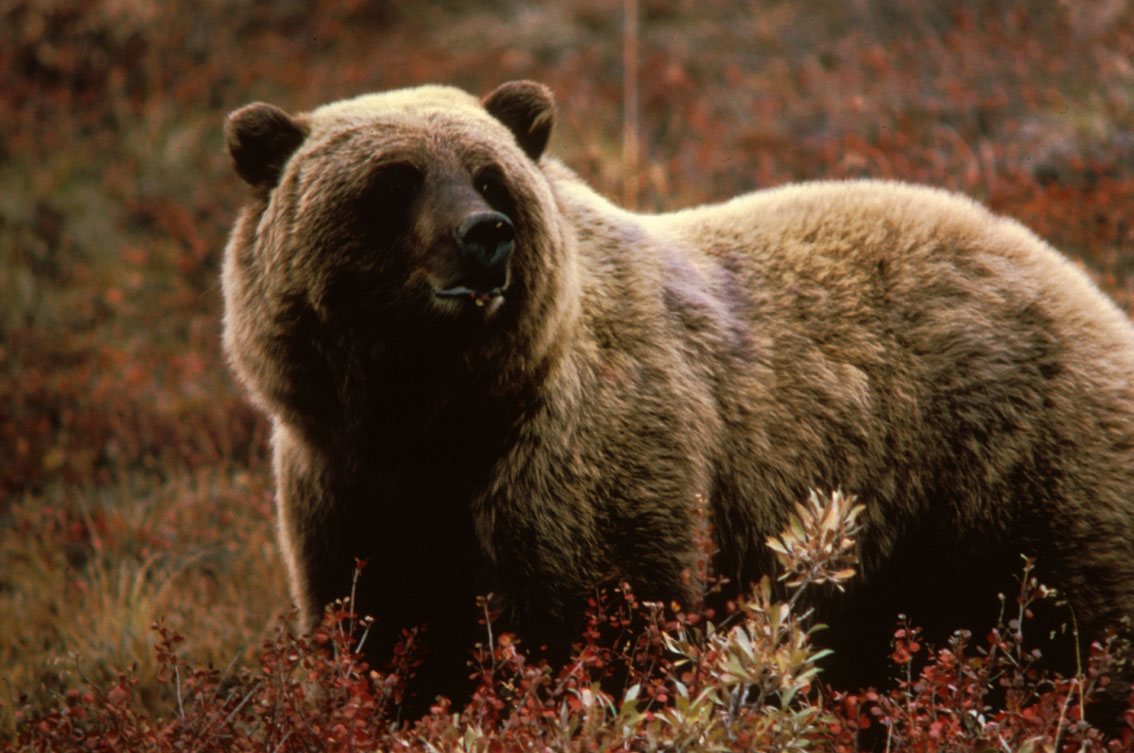
\includegraphics[width=\linewidth]{bear.jpg} % Figure image
	\caption{A majestic grizzly bear} % Figure caption
	\label{bear} % Label for referencing with \ref{bear}
\end{figure}

In hac habitasse platea dictumst. Vivamus eu finibus leo. Donec malesuada dui non sagittis auctor. Aenean condimentum eros metus. Nunc tempus id velit ut tempus. Quisque fermentum, nisl sit amet consectetur ornare, nunc leo luctus leo, vitae mattis odio augue id libero. Mauris quis lectus at ante scelerisque sollicitudin in eu nisi. Nulla elit lacus, ultricies eu erat congue, venenatis semper turpis. Ut nec venenatis velit. Mauris lacinia diam diam, ac egestas neque sodales sed. Curabitur eu diam nulla. Duis nec turpis finibus, commodo diam sed, bibendum erat. Nunc in velit ullamcorper, posuere libero a, mollis mauris. Nulla vehicula quam id tortor ornare blandit. Aenean maximus tempor orci ultrices placerat. Aenean condimentum magna vulputate erat mattis feugiat.

Quisque lacinia, purus id mattis gravida, sem enim fringilla erat, non dapibus est tellus pellentesque velit. Vivamus pretium sem quis leo placerat, at dignissim ex iaculis. Donec neque tortor, pharetra quis vestibulum id, tempus scelerisque mi. Cras in mattis est. Integer nec lorem rutrum, semper ligula bibendum, iaculis neque. Sed in nunc placerat, viverra dui in, fringilla sem. Sed quis rutrum magna, vitae pellentesque eros.

Praesent maximus mauris vitae nisl pulvinar, at tristique tortor aliquam. Etiam sit amet nunc in nulla vulputate sollicitudin. Aliquam erat volutpat. Praesent pharetra gravida cursus. Quisque vulputate lacus nunc. Integer orci ex, porttitor quis sapien id, eleifend gravida mi. Etiam efficitur justo eget nulla congue mattis. Duis commodo vel arcu a pretium. Aenean eleifend viverra nisl, nec ornare lacus rutrum in.

Vivamus pulvinar ac eros eu pellentesque. Duis nibh felis, sagittis sed lacus at, sagittis mattis nisi. Fusce ante dui, tincidunt in scelerisque ut, sagittis at magna. Fusce tincidunt felis et odio tincidunt imperdiet. Cras ut facilisis nisl. Aliquam vitae consequat metus, eget gravida augue. In imperdiet justo quis nulla venenatis accumsan. Aliquam aliquet consectetur tortor, at sollicitudin sapien porta sed. Donec efficitur mauris id rhoncus volutpat. Vestibulum ante ipsum primis in faucibus orci luctus et ultrices posuere cubilia Curae; Sed bibendum purus dapibus tincidunt euismod. Nullam malesuada ultrices lacus, ut tincidunt dolor. Etiam imperdiet quam eget elit tincidunt scelerisque. Curabitur ut ullamcorper dui. Cras gravida porta leo, ut lobortis nisl venenatis pulvinar. Proin non semper nulla.

Praesent pretium nisl purus, id mollis nibh efficitur sed. Sed sit amet urna leo. Nulla sed imperdiet sem. Donec ut diam tristique, faucibus ligula vel, varius est. In ipsum ligula, elementum vitae velit ac, viverra tincidunt enim. Phasellus gravida diam id nisl interdum maximus. Ut semper, tortor vitae congue pharetra, justo odio commodo urna, vel tempus libero ex et risus. Vivamus commodo felis non venenatis rutrum. Sed pulvinar scelerisque augue in porta. Sed maximus libero nec tellus malesuada elementum. Proin non augue posuere, pellentesque felis viverra, varius urna. Lorem ipsum dolor sit amet, consectetur adipiscing elit. Donec dignissim urna eget diam dictum, eget facilisis libero pulvinar.

Aliquam ex tellus, hendrerit sed odio sit amet, facilisis elementum enim. Suspendisse potenti. Integer molestie ac augue sit amet fermentum. Vivamus ultrices ante nulla, vitae venenatis ipsum ullamcorper sed. Phasellus gravida felis sapien, ac porta purus pharetra quis. Sed eget augue tellus. Nam vitae hendrerit arcu, id iaculis ipsum. Pellentesque sed magna tortor.

In ac tempus diam. Sed nec lobortis massa, suscipit accumsan justo. Quisque porttitor, ligula a semper euismod, urna diam dictum sem, sed maximus risus purus sit amet felis. Fusce elementum maximus nisi a mattis. Nulla vitae elit erat. Integer sit amet commodo risus, eget elementum nulla. Donec ultricies erat sit amet sem commodo iaculis. Donec euismod volutpat lacus, ut tempor est lacinia a. Vivamus auctor condimentum tincidunt. Praesent sed finibus urna. Sed pellentesque blandit magna et rhoncus.

Integer vel turpis nec tellus sodales malesuada a vel odio. Fusce et lectus eu nibh rhoncus tempus vel nec elit. Suspendisse commodo orci velit, lacinia dictum odio accumsan et. Vivamus libero dui, elementum vel nibh non, fermentum venenatis risus. Aliquam sed sapien ac orci sodales tempus a eget dui. Morbi non dictum tortor, quis tincidunt nibh. Proin ut tincidunt odio.

Pellentesque ac nisi dolor. Pellentesque maximus est arcu, eu scelerisque est rutrum vitae. Mauris ullamcorper vulputate vehicula. Praesent fermentum leo ac velit accumsan consectetur. Aliquam eleifend ex eros, ut lacinia tellus volutpat non. Pellentesque sit amet cursus diam. Maecenas elementum mattis est, in tincidunt ex pretium ac. Integer ultrices nunc rutrum, pretium sapien vitae, lobortis velit.

%----------------------------------------------------------------------------------------
%	BIBLIOGRAPHY
%----------------------------------------------------------------------------------------

\printbibliography[title={Bibliography}] % Print the bibliography, section title in curly brackets

%----------------------------------------------------------------------------------------

\end{document}
